\documentclass[11pt,a4paper]{article}

\usepackage[utf8]{inputenc}
\usepackage[T1]{fontenc}
\usepackage{amsmath,amssymb}
\usepackage{geometry}
\usepackage{booktabs}
\usepackage{hyperref}
\usepackage{xcolor}
\usepackage{listings}
\usepackage{microtype}
\usepackage{parskip}
\usepackage{graphicx}
\usepackage{float}
\graphicspath{{../SPECTRA/}}

\geometry{margin=2.5cm}

\hypersetup{
  colorlinks=true,
  linkcolor=blue!60!black,
  urlcolor=blue!60!black,
  citecolor=blue!60!black,
}

\lstset{
  language=Python,
  basicstyle=\ttfamily\small,
  keywordstyle=\color{blue!70!black}\bfseries,
  commentstyle=\color{gray},
  stringstyle=\color{orange!80!black},
  frame=single,
  breaklines=true,
  showstringspaces=false,
  columns=flexible,
}

\title{\textbf{Approximating Undulator Power with the Bending-Magnet Formula}\\[0.5em]
\large Theory, Validity, and Practical Implementation}
\author{M. Sanchez del Rio\\ESRF Grenoble France}
\date{\today}

% -----------------------------------------------------------------------
\begin{document}
\maketitle
\tableofcontents
\bigskip

% -----------------------------------------------------------------------
\section{Introduction}

Undulators produce quasi-monochromatic, highly collimated radiation through the constructive
interference of emission from successive magnetic periods.  Computing the exact spectrum
requires evaluating the full radiation integral (e.g.\ via SRW or SPECTRA), which is
numerically expensive and requires detailed knowledge of the electron beam emittance.

For \emph{power} estimates---particularly to assess thermal load on optical elements---the
bending-magnet (BM) approximation provides a fast, analytical alternative.  The key insight
is that in the wiggler limit ($K \gg 1$) successive poles radiate \emph{incoherently}, each
like an independent bending magnet.  The accuracy of this approximation and its practical
implementation are discussed in Section~\ref{sec:theory}.

% -----------------------------------------------------------------------
\section{Theoretical Motivation and Implementation}
\label{sec:theory}

The deflection parameter $K$ characterises the amplitude of the electron's transverse
oscillation in the periodic field $B_y = B_0 \cos(2\pi z / \lambda_u)$:
\begin{equation}
  K = \frac{e B_0 \lambda_u}{2\pi m_e c}
    \approx 0.9337\; B_0\,[\text{T}]\;\lambda_u\,[\text{cm}].
\end{equation}
The peak angular excursion of the electron is $\theta_{\max} = K/\gamma$, where
$\gamma = E_e / m_e c^2$ is the Lorentz factor.

Two radiation regimes can be considered:
\begin{itemize}
  \item \textbf{Undulator regime} ($K \lesssim 1$): $\theta_{\max} \lesssim 1/\gamma$.
        Emission cones from adjacent poles overlap; interference produces sharp harmonic
        peaks.  On-axis brightness scales as $N^2$.
  \item \textbf{Wiggler regime} ($K \gg 1$): $\theta_{\max} \gg 1/\gamma$.
        Emission fans are well separated; poles radiate independently.
        The spectrum approaches $2N$ times a bending-magnet spectrum.
\end{itemize}

\subsection{Power of the full emission of an insertion device}
The total radiated power of any insertion device with sinusoidal field
$B(z) = B_0\cos(2\pi z/\lambda_u)$ is \cite{kim1989}:
\begin{equation}
  \boxed{P\,[\text{W}] = 633\; B_0^2\,[\text{T}^2]\; L\,[\text{m}]\;
         E_e^2\,[\text{GeV}^2]\; I\,[\text{A}]}
  \label{eq:ptotal}
\end{equation}
where $L = N\lambda_u$ is the total device length.  The coefficient 633 incorporates the
sinusoidal average $\langle B^2\rangle = B_0^2/2$.  This formula is \emph{exact for any}
$K$; only the spectral \emph{distribution} depends on the regime.  In terms of $K$:
\begin{equation}
  P\,[\text{kW}] = 7.257\times10^{-5}\;
    \frac{E_e^2\,[\text{GeV}^2]\; K^2\; N}{\lambda_u\,[\text{m}]}\; I\,[\text{A}].
  \label{eq:ptotal_K}
\end{equation}
% The derivation of these formulas from the BM spectral formula is given in Section~\ref{sec:wigBM}.

% --- angular power density and slit power (Kim 1989) -------------------
\subsection{Power on a slit of an insertion device}
While the total power, Eq.\,(\ref{eq:ptotal}), fixes the overall scale, sizing a slit and
estimating the power it intercepts require the \emph{angular} distribution of the radiated
power.  Following Kim~\cite{kim1989}, the frequency-integrated power density factorises into
its on-axis value and a normalised angular shape function (Kim Eq.~4.61),
\begin{equation}
  \frac{d^2P}{d\Omega}(\theta,\psi)
    = \left.\frac{d^2P}{d\Omega}\right|_0 f_K(\gamma\theta,\gamma\psi),
  \label{eq:angfact}
\end{equation}
where $\theta$ and $\psi$ are the horizontal and vertical observation angles.  The on-axis
density, in practical units (Kim Eq.~4.63), is
\begin{equation}
  \left.\frac{d^2P}{d\Omega}\right|_0
    = 10.84\; B_0\,[\text{T}]\; E_e^4\,[\text{GeV}^4]\; I\,[\text{A}]\; N\; G(K)
    \quad [\text{W/mrad}^2],
  \label{eq:onaxis0}
\end{equation}
where the $2N$ factor for the $2N$ poles and the interference factor $G(K)$ are both absorbed
in the coefficient ($10.84 = 2\times5.42$, with $N$ written explicitly).  The interference
factor (Kim Eq.~4.60) is
\begin{equation}
  G(K) = \frac{K\!\left(K^6 + \tfrac{24}{7}K^4 + 4K^2 + \tfrac{16}{7}\right)}
              {\left(1+K^2\right)^{7/2}},
  \qquad G(K)\to 1 \ \text{for}\ K\gtrsim1.
  \label{eq:GK}
\end{equation}
The normalised angular function is valid for any $K$, satisfies $f_K(0,0)=1$, and reads
(Kim Eq.~4.62)
\begin{equation}
  f_K(\gamma\theta,\gamma\psi)
    = \frac{16K}{7\pi G(K)}\int_{-\pi}^{\pi}
      \frac{\sin^2\xi}{D^5}\Big[(1+X^2-Y^2)^2 + 4X^2Y^2\Big]\,d\xi,
  \label{eq:fK}
\end{equation}
with
\begin{equation}
  X = \gamma\psi,\qquad Y = K\cos\xi - \gamma\theta,\qquad D = 1 + X^2 + Y^2.
  \label{eq:XYD}
\end{equation}
The power transmitted by a rectangular slit subtending horizontal half-angle $\theta_0$ and
vertical half-angle $\psi_0$ is then the angular density integrated over the slit acceptance,
\begin{equation}
  \boxed{\;P_\text{slit}
    = \left.\frac{d^2P}{d\Omega}\right|_0
      \int_{-\theta_0}^{\theta_0}\!\!\int_{-\psi_0}^{\psi_0}
      f_K(\gamma\theta,\gamma\psi)\,d\theta\,d\psi\;}
  \label{eq:Pslit}
\end{equation}
with the angles expressed in mrad to match the units of Eq.\,(\ref{eq:onaxis0}).  Integrating
over all angles recovers the total power, Eq.\,(\ref{eq:ptotal}).  Equations
(\ref{eq:angfact})--(\ref{eq:Pslit}) are exact within the single-electron, zero-emittance
far-field approximation; the bending-magnet treatment developed below replaces the exact
$f_K$ by a cheaper incoherent-pole estimate suited to fast thermal-load calculations.
% -----------------------------------------------------------------------
\subsection{On-Axis Brilliance: Wiggler versus Undulator}

We have seen that the expressions for the total power emitted by the undulator
and wiggler are the same, when integrated over all the photon energies.
The headline distinction lies in how the radiation from successive magnet
periods combines, and it appears directly in the scaling with the number of
periods $N$. The two regimes are set by the deflection parameter $K$
which compares the electron's angular excursion $\sim K/\gamma$ with the natural
radiation opening angle $1/\gamma$.

When $K \lesssim 1$ (undulator regime), the angular excursion is comparable to $1/\gamma$, so the
radiation cones from all $N$ periods overlap and interfere. On resonance the
field \emph{amplitudes} add, and the on-axis angular flux density scales as
$N^2$:
%
\begin{equation}
  \left.\frac{dF}{d\Omega}\right|_{0}
  \approx 1.744\times10^{14}\, N^2 \, E^2[\mathrm{GeV}]\, I[\mathrm{A}]\, F_n(K)
  \quad [\mathrm{ph/s/mrad^2/0.1\%\,BW}].
\end{equation}
%
The interference also squeezes the radiation into a narrow central cone of
divergence
%
\begin{equation}
  \sigma_r' \approx \sqrt{\frac{\lambda}{2L}} \sim \frac{1}{\gamma\sqrt{N}},
  \qquad L = N\lambda_u,
\end{equation}
%
and concentrates the spectrum into sharp harmonic lines of bandwidth
$\Delta\lambda/\lambda \sim 1/(nN)$. Since brilliance divides the flux by the
source phase space,
%
\begin{equation}
  B \approx \frac{F}{4\pi^2\, \sigma_x \sigma_x' \, \sigma_y \sigma_y'},
\end{equation}
%
the small divergence and spectral concentration raise it further. The undulator
on-axis brilliance therefore scales roughly as $N^2$, with additional gains from
collimation and monochromaticity.

When $K \gg 1$ (wiggler regime), the angular swing $K/\gamma$ greatly exceeds $1/\gamma$, so the
cones from different poles point in different directions and the $2N$ poles
behave like independent bending magnets. The \emph{intensities} add, giving a
linear scaling:
%
\begin{equation}
  \left.\frac{dF}{d\Omega}\right|_{0}
  \approx 1.327\times10^{13}\, (2N)\, E^2[\mathrm{GeV}]\, I[\mathrm{A}]\, H_2(y)
  \quad [\mathrm{ph/s/mrad^2/0.1\%\,BW}].
\end{equation}
%
The radiation fans out horizontally over $\pm K/\gamma$ and forms a broadband
continuum (as for a bending magnet, but with higher critical energy). Both
effects enlarge the phase space and dilute the spectral density, so the
brilliance remains linear in $N$ with no interference enhancement.

For the same $N$, the undulator on-axis brilliance exceeds the wiggler's by
roughly a factor of $N$ (the ratio $N^2/N$), before even accounting for the
undulator's smaller divergence and narrower bandwidth---so in practice the gap
is often several orders of magnitude. The trade-off is that wigglers deliver
higher integrated flux and reach harder X-ray energies across a broad continuum,
whereas undulators dominate in brilliance, coherence, and tunable monochromatic
lines. Physically, the crossover is simply whether $K/\gamma$ is smaller than
(undulator) or much larger than (wiggler) the $1/\gamma$ radiation cone.

% -----------------------------------------------------------------------
\subsection{The undulator spectrum approximated by the wiggler}

In the wiggler limit, the undulator spectrum will show a multitude of peaks that tend
to merge and approaches $2N$ times the spectrum of an ``averaged"
single bending magnet.
%Even for moderate $K \sim 1$--2 this approximation reproduces integrated powers to within 20--30\,\%, sufficient for most thermal load estimates.
Figure~\ref{fig:spectral_power} compares the spectral power
computed by exact (SRW \cite{srw1998} in OASYS/XOPPY \cite{oasys} Undulator Spectrum), wiggler (WS in OASYS/XOPPY WS). Two
cases are compared, the full emission (or radiation collected in a very wide slit, in this case 30 x 10 mm$^2$ at 23~m) or in a ``small slit" as defined by the front end and primary slit (FE aperture is 1.8 x 1.0 mm$^2$ at 23 m). The cumulated power plots (Figure~\ref{fig:cumulated_power}) show that the total integrated power is the same full emission and emission on a small aperture  (equations~\ref{eq:ptotal} and \ref{eq:Pslit}, respectively). The cumulated power vs photon energy shows steps for the undulator and is very smooth for the wiggler, meaning that if some non-constant filtering is applied (when using attenuators and mirrors) the total integrated values will show differences. However, in cases where the filtering is not very selective, i.e., it is applied over undulator peaks that average out on the wiggler continuum, which appears for $K$ larger than one and is the case when the total power is higher, the use of a wiggler approximation may be reasonable for calculating the total power. This is exploited in this document.

\begin{figure}[htbp]
  \centering
  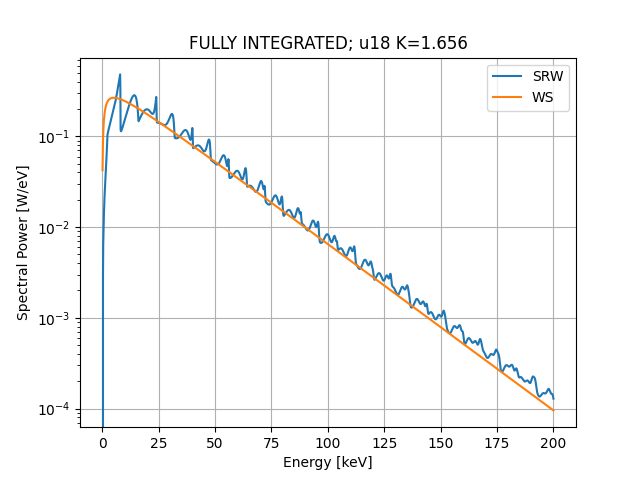
\includegraphics[width=0.45\textwidth]{figures/spectral_power_large_slits.png}
  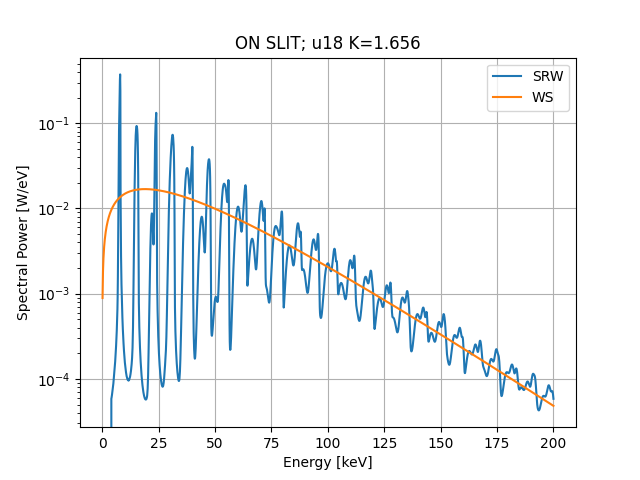
\includegraphics[width=0.45\textwidth]{figures/spectral_power_small_slits.png}
  \caption{Spectral power for a large slit (left, $30\times10$\,mm$^2$) and a small
           slit (right, $1.8\times1.0$\,mm$^2$) at 23\,m.}
  \label{fig:spectral_power}
\end{figure}

\begin{figure}[htbp]
  \centering
  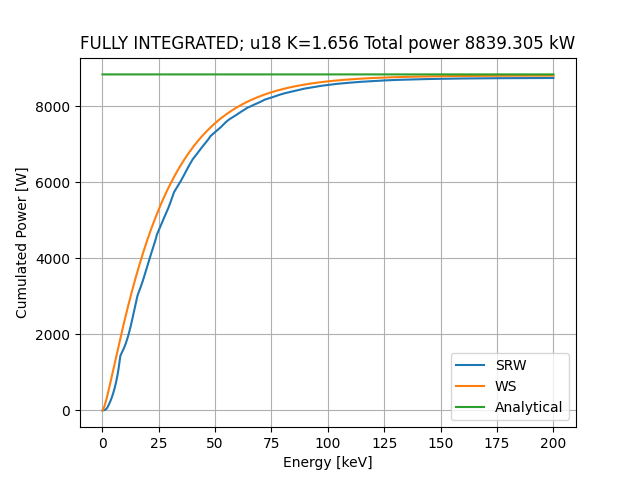
\includegraphics[width=0.45\textwidth]{figures/cumulated_power_large_slits.png}
  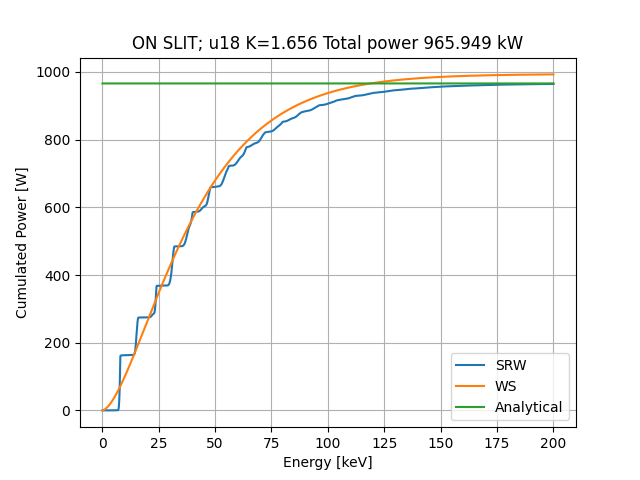
\includegraphics[width=0.45\textwidth]{figures/cumulated_power_small_slits.png}
  \caption{Cumulated power for a large slit (left, $30\times10$\,mm$^2$) and a small
           slit (right, $1.8\times1.0$\,mm$^2$) at 23\,m.
	   (For the small slit WS slightly overestimates the integrated power.)}
  \label{fig:cumulated_power}
\end{figure}

%Table~\ref{tab:validity} summarises the expected accuracy as a function of $K$.
%Residual errors at moderate $K$ arise from partial coherence between adjacent poles,
%concentration of power into discrete harmonics, and beam emittance effects neglected
%in the BM formula.
%
%\begin{table}[h]
%\centering
%\caption{BM approximation accuracy vs.\ deflection parameter.}
%\label{tab:validity}
%\begin{tabular}{ccl}
%\toprule
%$K$ range & Accuracy & Remarks \\
%\midrule
%$K < 0.5$   & poor ($>$50\,\%)      & Undulator regime; harmonic structure dominates \\
%$0.5$--$1$  & fair (20--50\,\%)     & Transition regime \\
%$1$--$2$    & good (10--30\,\%)     & Applicable for power estimates \\
%$K > 3$     & excellent ($<$10\,\%) & True wiggler regime; poles fully independent \\
%\bottomrule
%\end{tabular}
%\end{table}

% -----------------------------------------------------------------------
\subsection{Bending magnet radiation}

The angle-integrated BM spectral flux [ph/s/0.1\%bw/mrad] is \cite{green1976}:
\begin{equation}
  \Phi_\text{BM}(E,E_c) = 2.45706\times10^{13}\; E_e\,[\text{GeV}]\; I\,[\text{A}]
    \; G_1(E/E_c),
  \label{eq:phiBM}
\end{equation}
where $G_1(y) = y\int_y^\infty K_{5/3}(x)\,dx$ is a universal synchrotron function
and the critical energy is
\begin{equation}
  E_c\,[\text{keV}] = 0.6650\; E_e^2\,[\text{GeV}^2]\; B\,[\text{T}].
  \label{eq:ec}
\end{equation}
The exact integral of $G_1$ is obtained by exchanging the order of integration:
\begin{equation}
  \int_0^\infty G_1(y)\,dy
  = \int_0^\infty K_{5/3}(x)\frac{x^2}{2}\,dx
  = \Gamma\!\left(\tfrac{7}{3}\right)\Gamma\!\left(\tfrac{2}{3}\right)
  = \frac{8\pi}{9\sqrt{3}} \approx 1.6124.
  \label{eq:G1int}
\end{equation}
The power per unit horizontal angle is obtained by integrating Eq.\,(\ref{eq:phiBM})
over photon energy, using $dP/dE = \Phi_\text{BM}(E)\times E[\text{eV}]\times e / (0.001\times E[\text{eV}])$:
\begin{equation}
  \frac{dP}{d\theta}\,[\text{W/mrad}]
  = 2.45706\times10^{13} \times 1.602\times10^{-16}
    \times \frac{8\pi}{9\sqrt{3}} \times 665\;
    E_e^3\,[\text{GeV}]\; B\,[\text{T}]\; I\,[\text{A}]
  = 4.221\; E_e^3\; B\; I.
  \label{eq:dPdtheta}
\end{equation}
For a constant-field BM of arc length $L$, the total bending angle is
$\Delta\theta = L/\rho$ with $B\rho\,[\text{T\,m}] = 3.3356\,E_e\,[\text{GeV}]$,
so integrating Eq.\,(\ref{eq:dPdtheta}) over the arc gives:
\begin{equation}
  P_\text{BM} = \frac{4.221\times10^3}{3.3356}\; E_e^2\; B^2\; L\; I
  \approx 1266\; E_e^2\,[\text{GeV}^2]\; B^2\,[\text{T}^2]\; L\,[\text{m}]\; I\,[\text{A}]
  \quad[\text{W}].
  \label{eq:PBM}
\end{equation}

\subsubsection*{Independent derivation from the relativistic Larmor formula}

The same result can be derived from first principles using the relativistic Larmor
formula for a charge undergoing circular motion \cite{jackson1999} (eq.~14.31, SI units):
\begin{equation}
  P_e = \frac{e^2 c}{6\pi\epsilon_0}\cdot\frac{\gamma^4}{R^2} \quad [\text{W/electron}].
  \label{eq:larmor}
\end{equation}
For a beam of current $I$, the number of electrons simultaneously present in an arc
of length $L = R\Delta\theta$ is
\begin{equation}
  \bar{n} = \frac{I}{e}\cdot\frac{R\,\Delta\theta}{c},
\end{equation}
so the total beam power radiated in that arc is
\begin{equation}
  P = P_e\cdot\bar{n}
    = \frac{e^2 c}{6\pi\epsilon_0}\cdot\frac{\gamma^4}{R^2}
      \cdot\frac{I\,R\,\Delta\theta}{e\,c}
    = \frac{e}{6\pi\epsilon_0}\cdot\frac{\gamma^4\,\Delta\theta\,I}{R}.
  \label{eq:Parc}
\end{equation}
Substituting $R[\text{m}] = 3.3356\,E_e[\text{GeV}]/B[\text{T}]$ and
$\gamma = 1956.95\,E_e[\text{GeV}]$:
\begin{equation}
  P = \frac{e\,(1956.95)^4}{6\pi\epsilon_0\times 3.3356}
      \cdot E_e^3\,B\,\Delta\theta\,I.
\end{equation}
Evaluating the prefactor with $e=1.602\times10^{-19}$\,C,
$\epsilon_0=8.854\times10^{-12}$\,F/m:
\begin{equation}
  \frac{e\,(1956.95)^4}{6\pi\epsilon_0\times 3.3356}
  = \frac{1.602\times10^{-19}\times 1.4666\times10^{13}}
         {6\pi\times 8.854\times10^{-12}\times 3.3356}
  = \frac{2.350\times10^{-6}}{5.567\times10^{-10}}
  = 4221 \quad [\text{W\,rad}^{-1}\text{GeV}^{-3}\text{T}^{-1}\text{A}^{-1}],
\end{equation}
giving
\begin{equation}
  \boxed{\frac{dP}{d\theta} = 4221\cdot E_e^3[\text{GeV}^3]\cdot B[\text{T}]
         \cdot I[\text{A}] \quad [\text{W/rad}]}
  = 4.221\cdot E_e^3\cdot B\cdot I \quad [\text{W/mrad}].
  \label{eq:dPdtheta_larmor}
\end{equation}
This is identical to the spectral-formula result of $4.221$\,W/mrad
(Eq.\,\ref{eq:dPdtheta}).  The two routes --- relativistic Larmor
from first principles, and integration of the BM spectral formula with
$\int_0^\infty G_1\,dy = 8\pi/(9\sqrt{3})$ --- are therefore fully consistent.

% -----------------------------------------------------------------------
\subsection{The wiggler approximated by the BM}
\label{sec:wigBM}

In the wiggler limit the $2N$ half-periods each contribute an independent BM arc.
Two complementary approximations are derived below, valid in different aperture regimes.

\subsubsection*{Approach~1 --- arc integration (full aperture)}

The total power is obtained by applying Eq.\,(\ref{eq:dPdtheta}) locally along the
sinusoidal arc $B(s) = B_0\cos(2\pi s/\lambda_u)$, with $d\theta = |B(s)|/(B\rho)\,ds$:
\begin{align}
  P &= 2N \int_0^{\lambda_u/2}
       \frac{dP}{d\theta}\bigg|_{B(s)} \frac{|B(s)|}{B\rho}\,ds
  \nonumber\\
    &= \frac{2N \times 4.221\times10^3}{3.3356}\; E_e^2\; I
       \int_0^{\lambda_u/2} B_0^2\cos^2\!\left(\frac{2\pi s}{\lambda_u}\right)ds
  \nonumber\\
    &= \frac{2N \times 4.221\times10^3}{3.3356}\; E_e^2\; I \cdot
       \frac{B_0^2\,\lambda_u}{4}.
  \label{eq:approach1}
\end{align}
This gives coefficient $633$\,W\,T$^{-2}$\,m$^{-1}$\,GeV$^{-2}$\,A$^{-1}$, in
exact agreement with the LBL reference value \cite{kim1989}:
\begin{equation}
  \boxed{P\,[\text{W}] = 633\; B_0^2\,[\text{T}^2]\; L\,[\text{m}]\;
         E_e^2\,[\text{GeV}^2]\; I\,[\text{A}]},
  \label{eq:P633}
\end{equation}
where $L = N\lambda_u$.  The factor $\langle B^2\rangle = B_0^2/2$ from the sinusoidal
average enters naturally through the arc integral, recovering Eqs.\,(\ref{eq:ptotal})
and~(\ref{eq:ptotal_K}) stated above.
In practice Approach~1 is computed numerically: $N_\text{arc}$ BM spectra are evaluated
at local $E_c(s) = 665\,E_e^2\,|B(s)|$ and summed weighted by local $d\theta(s)$.
This yields a softer spectrum than the single peak-$B_0$ call of Approach~2, in better
agreement with WS for large apertures.

\textbf{Limitation:} Approach~1 integrates over all arc points regardless of horizontal
angle; it cannot account for a finite slit that selects only part of the fan.

\textbf{Application:} Approach~1 is used in OASYS/XOPPY Wiggler (full emission) and in
shadow4.

\subsubsection*{Approach~2 --- peak field with slit acceptance}

When a slit of width $w_h \times w_v$ at distance $D$ clips the horizontal fan, the
angular acceptances are $\Delta\theta_h^\text{slit} = w_h/D$ and
$\Delta\psi^\text{slit} = w_v/D$.  A narrow slit preferentially selects radiation from
the \emph{turning points} of the electron trajectory where $|B| \approx B_0$, so the
BM spectrum at peak critical energy $E_c(B_0)$ is appropriate.
The effective horizontal divergence is
\begin{equation}
  \Delta\theta_h^{\text{used}} = \min\!\left(\frac{2K}{\gamma},\,\frac{w_h}{D}\right),
  \label{eq:hdiv_used}
\end{equation}
and the slit-integrated flux is
\begin{equation}
  \Phi_{\text{slit}}(E) \approx 2N \cdot
    \Phi_\text{BM}\!\left(E,\,E_c(B_0)\right) \cdot \Delta\theta_h^{\text{used}}.
  \label{eq:approach2}
\end{equation}
Here $\Phi_\text{BM}$ must be the vertically-clipped flux integrated over $\psi \in [-w_v/(2D), +w_v/(2D)]$ (i.e. {\tt f\_psi=2} in {\tt sync\_ene()}).

When $\Delta\theta_h^\text{slit} \geq 2K/\gamma$ (full aperture), Approach~2
overestimates by exactly $4/\pi \approx 1.273$, because $dP/d\theta \propto B$
and the fan-average of the local field $B(\theta)=B_0\sqrt{1-(\theta \gamma / K)^2}$
is $\langle B\rangle = (\pi / 4) B_0$.

\subsubsection*{Hybrid implementation}

The two approaches are selected automatically based on the slit-to-fan ratio:
\begin{equation}
  \text{Use Approach~2 if } \frac{w_h}{D} < \frac{2K}{\gamma},
  \qquad
  \text{Use Approach~1 if } \frac{w_h}{D} \geq \frac{2K}{\gamma}.
  \label{eq:hybrid}
\end{equation}

\begin{center}
\begin{tabular}{llll}
\toprule
Approach & $E_c$ used & Horizontal weight & Best for  \\
\midrule
1 (arc integral) & local $E_c(s)$ & $\int|B(s)|ds/(B\rho)$ & total power  \\
2 (peak field)   & $E_c(B_0)$ & $\min(w_h/D,\;2K/\gamma)$ & slit power \\
\bottomrule
\end{tabular}
\end{center}

Note that the hybrid switch (Eq. \ref{eq:hybrid}) has a 27\% discontinuity at
$w_h/D=2K/\gamma$:
Approach 2 hits the boundary at 1.273$\times$ exact while Approach 1 is exact.
A smooth alternative is the elliptical weighting:
\begin{equation}
\Delta\theta_h^\text{eff} = \frac{K}{\gamma}\left[\arcsin u + u\sqrt{1-u^2}\right], \qquad u = \min\!\left(1,\ \frac{w_h\gamma}{2DK}\right)
\label{eq:elliptic}
\end{equation}
which  $\rightarrow w_h/D$ for small slits (the rectangle is fine near the axis,
since $B(\theta)\approx B_0$
there) and $ \rightarrow (\pi/2)K/\gamma$
at full aperture (exact total power). Both limits are easily verified, and for the CPMU18 slit ($u=0.28$) Eq.\,(\ref{eq:elliptic}) differs from the rectangle by only 1.3\% --- confirming why the small-slit results were already excellent.


% -----------------------------------------------------------------------
\section{Summary and Recommendations}

\begin{itemize}
  \item \textbf{Approach~1 (arc integration)}: integrating the BM spectral formula
        locally along the sinusoidal arc, weighted by the local bending angle
        $d\theta = |B(s)|ds/(B\rho)$, gives the exact total power
        $P = 633\,B_0^2\,L\,E_e^2\,I$\,[W] with a naturally averaged spectral shape.
        This is the recommended approach for \textbf{full-aperture power}.
  \item \textbf{Approach~2 (peak field)}: using the peak field $B_0$ and
        $E_c(B_0)$ with $\Delta\theta_h^\text{used} = \min(2K/\gamma,\,w_h/D)$
        gives near-exact agreement with SRW ($\sim$2\,\%) for a slit that clips
        the horizontal fan.  This is the recommended approach for
        \textbf{slit-integrated power}. This is the approach to be used for the
		wattdog ID11 calculations, where the maximum aperture is 1.8$\times$1.0 mm$^2$ at 23~m.
  \item A \textbf{hybrid implementation} selects automatically between the two
        approaches based on whether the slit is narrower or wider than $2K/\gamma$. The elliptical correction of Eq.\,(\ref{eq:elliptic}) for smoothing the transition has not been implemented.
  \item The approximation \textbf{fails for spectral shape}: it produces a smooth
        BM-like continuum and misses the harmonic structure entirely.  It should
        \emph{not} be used for monochromatic flux, rocking-curve calculations, or
        any application requiring spectral detail.
\end{itemize}

% -----------------------------------------------------------------------
\begin{thebibliography}{9}

\bibitem{jackson1999}
J.~D. Jackson,
\textit{Classical Electrodynamics}, 3rd ed.,
Wiley, New York, 1999.

\bibitem{green1976}
G.~K. Green,
\textit{Spectra and optics of synchrotron radiation},
BNL Report 50522, Brookhaven National Laboratory, 1976.

\bibitem{sokolov1968}
A.~A. Sokolov and I.~M. Ternov,
\textit{Synchrotron Radiation},
Akademik-Verlag, Berlin, 1968.

\bibitem{kim1989}
K.-J. Kim,
\textit{Characteristics of synchrotron radiation},
AIP Conf.\ Proc.\ \textbf{184}, 565 (1989).

\bibitem{srw1998}
O.~Chubar and P.~Elleaume,
\textit{Accurate and Efficient Computation of Synchrotron Radiation in the Near Field Region},
Proc.\ EPAC 1998, p.~1177.

\bibitem{srxraylib}
M.~Sanchez del Rio and L.~Rebuffi,
\texttt{srxraylib}: synchrotron radiation tools,
\url{https://github.com/oasys-kit/sr-xraylib}.

\bibitem{oasys}
M.~Sanchez del Rio and L.~Rebuffi,
\texttt{OASYS}: OrAnges SYnchrotron Suite,
\url{https://oasys-kit.github.io/}.

\end{thebibliography}

\end{document}

